\documentclass[../main.tex]{subfiles}

\begin{document}
%%%%%%%%%%%%%%%%%%%%%%%%%%%%%%%%%%%%%%%%%%%%%%%%%%%%%%%
%   New Chapter                                       %
%%%%%%%%%%%%%%%%%%%%%%%%%%%%%%%%%%%%%%%%%%%%%%%%%%%%%%%

\chapter{Non-Negative Matrix Factorization}
This chapter discusses a variant of matrix factorization, where for some reason we want the entries of our model to be non-negative, and we will try to understand how does this assumption change our problem. We will start from a classical motivation from the field of Natural Language Processing (NLP), namely topic modeling, and then introduce two important approaches, with a brief interlude to review the Expectation Maximization (EM) algorithm. Finally, we will discuss the non-negative matrix factorization (NMF) problem from a more general perspective.
\section{Motivation}
Given a corpus of text documents, like web pages, a usual challenge in NLP is to find a low-dimensional representation in semantic space of topics or concepts for the documents. This is also known as \emph{topic models}, where we want to find these topics in the data set and represent documents with regard to these topics. 
\par From a probabilistic view, we can address this problem by building a predictive model for each document and predicting additional words for this document. In another word, given some observed words we try to predict the probabilities for additional words. This approach comes from the intuition that model with high prediction power should extract interesting structures of the data. Concretely, we can try to maximize the log-likelihood of predicting words in the document, which gives exactly the idea of \emph{probabilistic Latent Semantic Analysis (pLSA)}. \emph{Latent Dirichlet Allocation (LDA)} improves pLSA by exploiting the ability to generate new data from a Bayesian point of view. pLSA is closely related to NMF and will be discussed again in the last section of this chapter.
\par Before pLSA, it's useful to introduce some concepts and commonly-used pre-processing. The \emph{vocabulary} is the set of all "meaningful" words in a language and is extracted from corpus documents via \emph{tokenization} (also known as word segmentation), which segments the text or document into a sequence of strings (words) based on certain rules. For human languages, the vocabularies are usually with large cardinality (say 1-100 million). \emph{Term filtering} and \emph{term normalization} are also popularly applied, where the first one excludes stop words like "the" or "at" and infrequent words, misspellings, etc; the second one reduces words to stems (\emph{stemming}) like reducing "argue" and "argues" to the stem "arg".
\par As far as what the topicality is concerned of what the document is about, we can make an assumption to use \emph{Bag-of-Word (BoW) representations} for documents, which ignore the order of word in sentences and simplify the problem to a matrix problem. The BoW representation reduces the whole data set to co-occurrence counts (Figure \ref{fig_4_1}), where in this case the context of each word is the entire document, and each document is then a M-dimensional vector of counts. Recall that M is usually very large, then the document vectors are very sparse. Note that the sparsity here is different from the one in the rating task, where the sparsity comes from the lack of observation. Here the zeros simply mean zero counts and are actually observed values.
\par It might seem to be a reasonable approach to make prediction based on this co-occurrence count matrix, but since it's very sparse it will give zero probabilities to unseen words in a document. For a predictive model, we want to do better.
\begin{figure}[h] 
	\centering 
	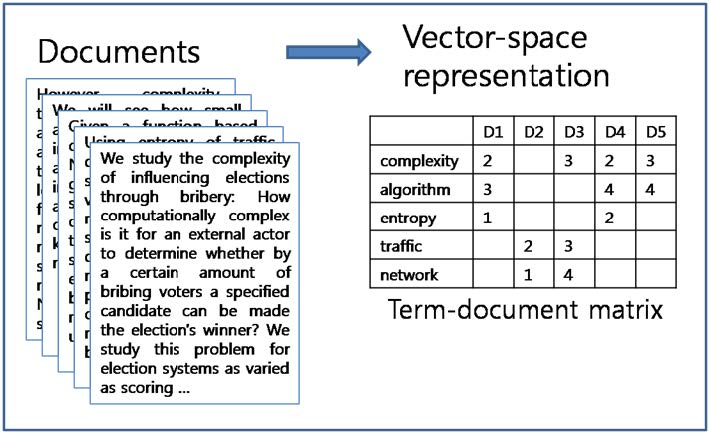
\includegraphics[width=8cm]{fig_4_1.jpg} 
	\caption{Bag-of-Word embedding}\label{fig_4_1}
\end{figure}
\section{Probabilistic Latent Semantic Analysis}
pLSA identifies topics with characteristic distributions over words, which are the model parameters, and models each document as a \textbf{mixture of topics}. Note that the mixing weights are not the uncertainties about certain "correct" topic but show that the document belongs to multiple topics with different "importance". For example, a report about soccer world cup 2022 might contains words from soccer vocabulary (e.g. "teams", "play", "match") in a sense of distribution and words from political vocabulary (e.g. "labor", "corruption", "president") in a sense of distribution. The goal is to discover topics in an unsupervised fashion.
\subsection{Basic Model}
As a predictive model, pLSA samples words in a two-stage manner:
\begin{enumerate}
	\item Sample topic from the mixtures for each token/word.
	\item Sample token/word, given sampled topic
\end{enumerate}
\par As illustrated in Figure \ref{fig_4_2}, different colors correspond to different topics. Given a document $d$, we first sample topics $z_i$ for every position $i$ in the document, and then sample a word $w_i$ conditioning on the topic $z_i$ of that position.
\begin{figure}[h] 
	\centering 
	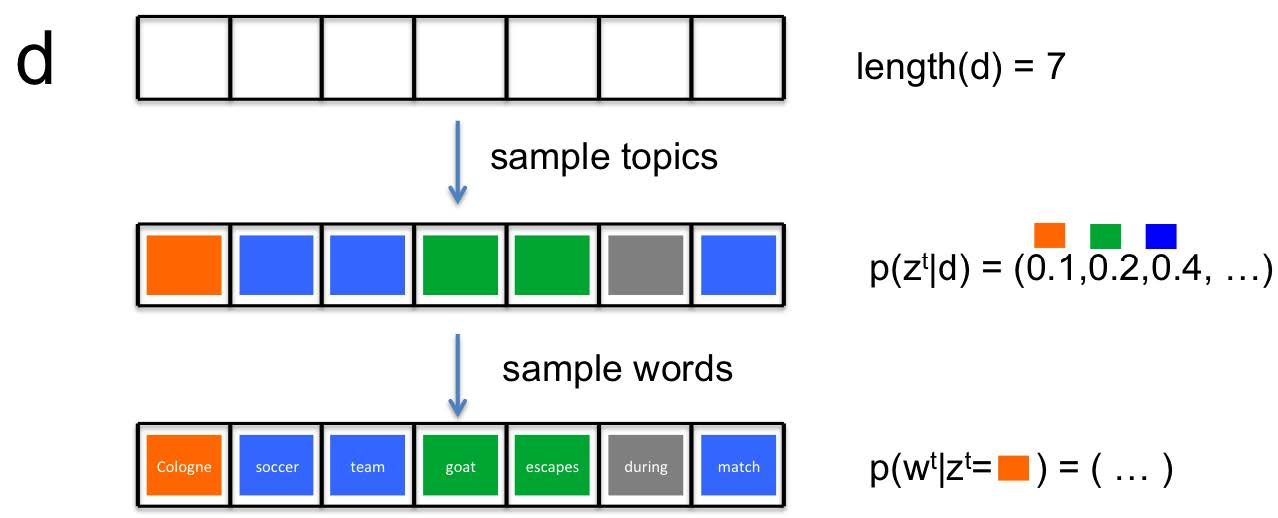
\includegraphics[width=8cm]{fig_4_2.jpg} 
	\caption{Two-stage sampling of pLSA}\label{fig_4_2}
\end{figure}
\par The model parameters are tied up together with this two-stage sampling:
\begin{enumerate}
	\item Each document has a specific mix of topics: $p(z|d)$.
	\item Each topic has a specific distribution of words: $p(w|z)$.
\end{enumerate}
\par Given the model parameters, we can compute the log-likelihood of observed data and use some criterion to evaluate how well our model performs. Specifically, we can get the occurrence (probability) of word $w$ in context/document $d$ (also known as context model) by marginalizing out topic $z$ from the conditional joint distribution given $d$:
\begin{equation}\label{eq_4_word_prob}
p(w|d)=\sum_{z=1}^{K}p(w,z|d)=\sum_{z=1}^{K}p(w|z,d)p(z|d) = \sum_{z=1}^{K}p(w|z)p(z|d)
\end{equation}
where we identify topics with integers $z\in \{1,\dots,K\}$ ($K$: pre-specified), and word $w$ is related to a fixed "slot", i.e. fixed position in the document, and has an identical distribution for every slot. In the last equality above, we made a conditional independence assumption $w\perp d\ |\ z$ meaning that topics represent regularities common to the entire collection.
\begin{remark}
	As mentioned above, we need to pre-specify the topic number $K$ for pLSA. However, we need to be careful about the interpretability of our model on these "topics". For example, if we apply pLSA with $K=4$ on data collected from 4 topics (say "sports", "politics", "music", and "science"), we may expect our pLSA model to find these topics, but with $K=3$ the "meaning" of topics found by our model may be a lot more unpredictable. 
\end{remark}
\par With (\ref{eq_4_word_prob}) and an additional assumption that every word in a document is independent of each other, the data can be represented in two possible views:
\begin{itemize}
	\item Summarize data into co-occurrence counts ${\bf X}=x_{ij}$ (number of occurrences of $w_j$ in document $d_i$)
	\item Alternatively: multiset $\mathcal{X}$ over index pair $(i,j)$, e.g. 
	$$\mathcal{X} = \{(1,1), (1,1), (1, 2),\dots\}$$
\end{itemize} 
The log-likelihood, therefore, is
\begin{equation}\label{eq_4_log_l}
l({\bf U},{\bf V})=\sum_{i,j}x_{ij}\log p(w_j|d_i)=\sum_{(i,j)\in \mathcal{X}}\log \sum_{z=1}^{K} \underbrace{p(w_j|z)}_{=:v_{zj}}\underbrace{p(z|d_i)}_{=:u_{zi}}
\end{equation}
where $u_{zi}\geq 0$ and $v_{zj}\geq 0$ are model parameters. Since they are probability distributions, we further require constraints:
\begin{equation*}
\sum_z u_{zi}=1\ (\forall i),\ \sum_j v_{zj}=1\ (\forall z)
\end{equation*}
\par A natural attempt is to optimize (\ref{eq_4_log_l}) via gradient descent, but the sum of probabilities inside the $\log$ can cause problems (no explicit optimal solution anymore and expensive computation cost for large $K$ in gradient descent methods). In the following, we will address the problem from another view, namely the Expectation Maximization, which iteratively optimizes a lower bound of the original objective function. Since it's a very useful algorithm and is closely related to another topic we will meet in the sequel, the k-means algorithm, we will introduce more of EM in details in the next section, while it might be out of the scope of this course.
\subsection{Expectation Maximization for pLSA}
EM deals with the hardness of maximization of the original log-likelihood function by assuming latent variables and bring them back to play, which is known as complete data model. Denote all observed variables (i.e. words in topic model) as ${\bf X}$, all latent variables as ${\bf Z}$, and model parameters as $\theta$. Then, $\{{\bf X, Z}\}$ represents the complete data set, while $\{{\bf X}\}$ is called incomplete data set. In this case, we shall suppose that optimization of the $p({\bf X}|\theta)$ is hard but easy for $p({\bf X, Z}|\theta)$. This will be discussed in detail in the next section.
\par In pLSA, we introduce missing data $Q_{zij}\in\{0,1\}$ indicating that $w_j$ in $d_i$ is generated via $z$. Note that by construction: $\sum_{z}Q_{zij}=1$. Then this naturally yields corresponding variational parameters (latent variables), which is a distribution over $z$:
\begin{equation*}
q_{zij}=\mathbb{P}(Q_{zij}=1),\ \sum_{z} q_{zij}=1
\end{equation*}
With $q_{zij}$, we can lower bound $\log p(w_j|d_i)$ in (\ref{eq_4_log_l}) via Jensen's inequality. First re-write it into a convex combination, using that $q_{zij}\geq 0,\ \sum_{z} q_{zij}=1$:
\begin{equation*}
\log p(w_j|d_i) = \log \sum_{z=1}^{K} u_{zi}v_{zj} =  \log \sum_{z=1}^{K} q_{zij}\frac{u_{zi}v_{zj}}{q_{zij}}
\end{equation*}
Then since $\log(\cdot)$ is a concave function, Jensen's inequality gives:
\begin{equation}\label{eq_4_lwb}
\log p(w_j|d_i) =\log \sum_{z=1}^{K} q_{zij}\frac{u_{zi}v_{zj}}{q_{zij}} \geq \sum_{z=1}^{K} q_{zij}[\log u_{zi} + \log v_{zj} - \log q_{zij}]
\end{equation}
Optimizing over $q$ for fixed $u_{zi},v_{zj}$ maximizes the lower bound (\textbf{Expectation Step}). To solve for optimal $q$, we can apply Lagrangian:
\begin{equation*}
\mathcal{L}(q, \lambda) = \sum_{z=1}^{K} q_{zij}[\log u_{zi} + \log v_{zj} - \log q_{zij}] + \lambda (\sum_{z} q_{zij}-1)
\end{equation*}
Applying the first order optimality condition, we get
\begin{equation*}
\lambda + (\log u_{zi}v_{zj} - \log q_{zij} -1) \overset{set}{=}0.
\end{equation*}
Plugging this back in the normalization constraint we get
\begin{equation*}
q_{zij} = \frac{u_{zi}v_{zj}}{\sum_{z=1}^{K}u_{zi}v_{zj}} = \frac{p(w_j|z)p(z|d_i)}{\sum_{z=1}^{K}p(w_j|z)p(z|d_i)}
\end{equation*}
which turns out to be the posterior of $Q_{zij}$ under current model ($\{u_{zi},v_{zj}\}$). The interpretation of the Expectation step is clear: if given $u_{zi},v_{zj}$ we can solve for the optimal $q$. But since we don't know the true model parameters in advance, we need to do it iteratively with the following \textbf{Maximization Step}, which solves for the optimal parameters with fixed $q$. First apply lower bound (\ref{eq_4_lwb}) to the log-likelihood (\ref{eq_4_log_l}):
\begin{equation*}
l({\bf U},{\bf V}) \geq \sum_{i,j}x_{ij} \sum_{z=1}^{K} q_{zij}[\log u_{zi} + \log v_{zj} - \log q_{zij}]
\end{equation*}
Then again we can apply Lagrangian to solve for optimal $u_{zi}$ and $v_{zj}$. With a similar derivation, we get
\begin{equation*}
u_{zi}=\frac{\sum_{j}x_{ij}q_{zij}}{\sum_{j}x_{ij}},\quad v_{zj}=\frac{\sum_{i}x_{ij}q_{zij}}{\sum_{i,l}x_{il}q_{zil}}
\end{equation*}
where in the first equality we used $\sum_{z} q_{zij}=1$. Note that the denominators of the two expressions differs simply because $u_{zi}$ is a distribution over $z$ and $v_{zj}$ is a distribution over $j$. Also, we see that the numerators are simple weighted counts, and the denominators ensure proper normalization.
\par EM for MLE in pLSA gives a simple alternating scheme for finding a solution and is guaranteed to converge. However, EM is not guaranteed to find global optimum.
\section{Expectation Maximization in a section}\label{sec_4_EM}
This section is not relevant to this course and is written for my personal interests. So feel free to skip it! The content mainly comes from chapter 9 of one of my favorite books, \emph{Pattern Recognition and Machine Learning} by Christopher M. Bishop. I recommend ones who are interested in more materials to read the corresponding chapters.
\subsection{K-means Clustering}
One of the most popular clustering methods is k-means algorithm. Given $x_1,\dots,x_n\in \mathbb{R}^d$, the k-means algorithm partitions the data points into k disjoint "groups" $S_1,\dots,S_k$ with centers $\mu_1,\dots,\mu_k\in \mathbb{R}$, which can be seen as prototypes of each "group". In another word, k-means defines the following optimization problem:
\begin{equation*}
\min_{\{S_k\},\{\mu_k\}}\sum_{k=1}^{K}\sum_{n\in S_k}\|x_n-\mu_k\|^2
\end{equation*}
or equivalently
\begin{equation*}
\min_{\{r_{nk}\},\{\mu_k\}}\sum_{k=1}^{K}\sum_{n=1}^{N}r_{nk}\|x_n-\mu_k\|^2
\end{equation*}
where $r_{nk}\in \{0,1\}$ is a binary indicator variable describing which of the $K$ cluster the data $x_n$ is assigned to. Since directly optimizing k-means objective is NP-hard, we usually apply an iterative scheme, which is also known as Lloyd's algorithm:
\begin{itemize}
	\item Given centers $\mu_1,\dots,\mu_K$, assign each point to the closest center:
	\begin{equation*}
	r_{nk}=\begin{cases}
	1& \text{if }k=\arg\min_j\|x_n-\mu_j\|^2\\
	0& \text{otherwise.}
	\end{cases}
	\end{equation*}
	\item Given all the assignments, find the optimal centers:
	\begin{equation*}
	\mu_k = \frac{1}{|S_k|}\sum_{n\in S_k}x_n.
	\end{equation*}
\end{itemize}
We shall see that these two stages of updating $r_{nk}$ and updating $\mu_k$ correspond to the E steps and M steps of the EM algorithm, respectively.
\subsection{Mixtures of Gaussians}
We now turn to a formulation of Gaussian mixtures in terms of discrete latent variables, which will serve to motivate the EM algorithm. A Gaussian mixture distribution can be written in a form of linear superposition of Gaussians:
\begin{equation*}
p({\bf x})=\sum_{k=1}^{K} \pi_k \mathcal{N}({\bf x}|\bm{\mu}_k, {\bf\Sigma}_k).
\end{equation*}
Let us introduce a K-dimensional binary random variable ${\bf z}$ satisfying that $z_k\in \{0,1\}$ and $\sum_k z_k=1$. Then we can define the joint distribution $p({\bf x,z})$ using a marginal distribution $p({\bf z})$ and a conditional distribution $p({\bf x}|{\bf z})$. $p({\bf z})$ is specified in terms of the mixing coefficients $\pi_k$, such that
\begin{equation*}
p(z_k=1)=\pi_k \in [0,1],\ \sum_k\pi_k=1
\end{equation*}
which yields
\begin{equation*}
p({\bf z})=\prod_{k}\pi_k^{z_k}.
\end{equation*}
On the other hand, the conditional distribution of ${\bf x}$ given a specific ${\bf z}$, note that ${\bf z}$ only has K different states, is given by
\begin{equation*}
p({\bf x}|z_k=1)=\mathcal{N}({\bf x}|\bm{\mu}_k,{\bf \Sigma}_k)
\end{equation*}
which is equivalent to
\begin{equation*}
p({\bf x}|{\bf z}) = \prod_k \mathcal{N}({\bf x}|\bm{\mu}_k,{\bf \Sigma}_k)^{z_k}.
\end{equation*}
The marginal distribution of ${\bf x}$ is then obtained by summing the joint distribution $p({\bf x,z})=p({\bf z})p({\bf x}|{\bf z})$ over all possible states of ${\bf z}$:
\begin{equation*}
p({\bf x}) = \sum_z p({\bf z})p({\bf x}|{\bf z}) =  \sum_z \prod_k (\pi_k \mathcal{N}({\bf x}|\bm{\mu}_k,{\bf \Sigma}_k))^{z_k} = \sum_{k} \pi_k \mathcal{N}({\bf x}|\bm{\mu}_k, {\bf\Sigma}_k).
\end{equation*}
We have therefore found an equivalent formulation of the Gaussian mixture involving an explicit latent variable. This allow us to work with the joint distribution $p({\bf x, z})$ instead of $p({\bf x})$, which will lead to significant simplifications. Another quantity that will play an important role is $p({\bf z|x})$. We use $\gamma(z_k)$ to denote $p(z_k=1|{\bf x})$, whose value can be found using Bayes' theorem:
\begin{align*}
\gamma(z_k) \equiv p(z_k=1|{\bf x})= \frac{p(z_k=1)p({\bf x}|z_k=1)}{\sum_i p(z_i=1)p({\bf x}|z_i=1)}= \frac{\pi_k \mathcal{N}({\bf x}|\bm{\mu}_k, {\bf\Sigma}_k)}{\sum_{i} \pi_i \mathcal{N}({\bf x}|\bm{\mu}_i, {\bf\Sigma}_i)}.
\end{align*}
$\gamma(z_k)$ has an interpretation as the \emph{responsibility} that component $k$ takes for "explaining" the observation ${\bf x}$. 
\par Now we represent the data that we want to model with Gaussian mixtures by ${\bf X}\in \mathbb{R}^{N\times D}$ with the $n^{\text{th}}$ row is given by ${\bf x}_n^T$, and the latent variables by ${\bf Z}\in \mathbb{R}^{N\times K}$ with the $n^{\text{th}}$ row ${\bf z}_n^T$. Assume that the data points are independently drawn from the distribution, the log-likelihood therefore is given by
\begin{equation}\label{eq_4_log_l_gm}
\ln p({\bf X}|\bm{\pi},\bm{\mu},{\bf \Sigma}) = \sum_{n=1}^{N}\ln \left\{\sum_{k=1}^{K} \pi_k \mathcal{N}({\bf x}|\bm{\mu}_k, {\bf\Sigma}_k)\right\}.
\end{equation}
The difficulty of maximizing (\ref{eq_4_log_l_gm}) arises from the presence of the summation over $k$ that appears inside the logarithm. If we set the derivative to zero, we can no longer get a close form solution.
\subsection{EM for Gaussian mixtures}
\emph{Expectation-maximization} is an elegant and powerful method for finding maximum likelihood solutions for models with latent variables. First we will discuss EM in the context of Gaussian mixtures, and later in a more general view.
\par The conditions that must be satisfied for an optimal solution is the first order optimality condition. Setting the derivatives of (\ref{eq_4_log_l_gm}) with respect to $\bm{\mu}_k$ and ${\bf \Sigma}_k$ to zero, we obtain
\begin{align}
\label{eq_4_mu}&\frac{\partial (\ref{eq_4_log_l_gm})}{\partial \bm{\mu}_k}=0\Rightarrow \bm{\mu}_k = \frac{1}{N_k}\sum_{n=1}^{N}\gamma(z_{nk}){\bf x}_n\\
\label{eq_4_sigma}&\frac{\partial (\ref{eq_4_log_l_gm})}{\partial {\bf \Sigma}_k}=0\Rightarrow {\bf \Sigma}_k=\frac{1}{N_k}\sum_{n=1}^{N}\gamma(z_{nk}) ({\bf x}_n-\bm{\mu}_k)({\bf x}_n-\bm{\mu}_k)^T\\
\label{eq_4_gamma}&N_k = \sum_{n=1}^{N}\gamma(z_{nk}), \quad\gamma(z_{nk}) = \frac{\pi_k \mathcal{N}({\bf x}_n|\bm{\mu}_k,{\bf \Sigma}_k)}{\sum_i\pi_i \mathcal{N}({\bf x}_n|\bm{\mu}_i,{\bf \Sigma}_i)} 
\end{align}
where we have assumed that ${\bf \Sigma}_k$ is invertible for all $k$, and $N_k$ has a interpretation as the effective number of point assigned to cluster $k$. From the form of this solution we see that $\bm{\mu}_k$ and ${\bf \Sigma}_k$ are weighted version of mean and variance of the data set, and the weighting factor for ${\bf x}_n$ is given by the posterior probability $\gamma(z_{nk})$ that component $k$ was responsible for generating ${\bf x}_n$.
\par Finally, we maximize (\ref{eq_4_log_l_gm}) w.r.t. the mixing coefficients $\pi_k$. Note that $\pi_k$ needs to be non-negative and normalized. We use a Lagrange multiplier to force the normalization constraint and show that the solution satisfies the non-negative constraint automatically. Define the following Lagrangian
\begin{equation*}
\mathcal{L}=\ln p({\bf X}|\bm{\pi},\bm{\mu},{\bf \Sigma}) + \lambda\left(\sum_k \pi_k-1\right).
\end{equation*}
Set it's derivative to zero w.r.t. $\pi_k$ and use the normalization constraint we obtain
\begin{equation}\label{eq_4_pi}
\pi_k = \frac{N_k}{N} 
\end{equation}
which has a clear interpretation as the average responsibility that component $k$ takes for explaining the data points. It is worth emphasizing that the results (\ref{eq_4_mu}), (\ref{eq_4_sigma}), and (\ref{eq_4_pi}) are not closed form solutions for the model parameters because of the dependency of the responsibilities $\gamma(z_{nk})$ on these parameters. However, these results suggest a simple iterative scheme for finding a solution, which we will see turns out to be an instance of the EM algorithm. 
\par We first initialize all the model parameters, and then alternate between the following two updates until some conditions are satisfied:
\begin{itemize}
	\item  \textbf{E (expectation) step}: Use the current model parameters $\{\bm{\pi}, \bm{\mu}, {\bf \Sigma}\}$ to evaluate the posterior probabilities/responsibilities $\gamma(z_{nk})$ via (\ref{eq_4_gamma}).
	\item  \textbf{M (maximization) step}: Use the updated responsibilities $\gamma(z_{nk})$ to re-estimate model parameters $\{\bm{\pi}, \bm{\mu}, {\bf \Sigma}\}$ via (\ref{eq_4_mu}), (\ref{eq_4_sigma}), and (\ref{eq_4_pi}).
\end{itemize}
We shall see that in each update the parameters resulting from an E step followed by an M step is guaranteed to increase the log-likelihood function. Since the log-likelihood function is always upper-bounded by 0, EM is therefore guaranteed to converge in general since EM maximizes a lower bound for the log-likelihood in each step.
\subsection{An Alternative View of EM}\label{sec_4_em_km_compare}
In this section, we will discuss th EM algorithm in a more general setting. The goal of the EM algorithm is to find maximum likelihood solutions for models having latent variables. We denote the set of all observed data by ${\bf X}$ with the $n^{\text{th}}$ row representing ${\bf x}_n^T$, and similarly we denote the set of all latent variables by ${\bf Z}$ with a corresponding row ${\bf z}_n^T$. Given the set of all model parameters denoted by $\bm{\theta}$, the log-likelihood of ${\bf X}$ is
\begin{equation*}
\ln p({\bf X}|\bm{\theta}) = \ln \left(\sum_{\bf Z} p({\bf X,Z}|\bm{\theta}) \right).
\end{equation*}
The hardness of optimizing this objective arises from summation over the latent variables inside the logarithm. Now suppose that, for each observation ${\bf X}$, we were told the corresponding value of the latent variable {\bf Z}. We shall call $\{{\bf X, Z}\}$ the \emph{complete} data set, and refer to the actual observed data ${\bf X}$ as \emph{incomplete}. We shall suppose that maximization of the complete-data log likelihood function $\ln p({\bf X,Z}|\bm{\theta})$ is straightforward.
\par In practice, we are not given the complete data set $\{{\bf X, Z}\}$, and our knowledge of the values of the latent variables ${\bf Z}$ is given only by the posterior distribution $p({\bf Z}|{\bf X},\bm{\theta})$. Because we cannot use the complete-data log-likelihood, we consider instead its expected value under the posterior distribution of the latent variable, which corresponds to the E step of the EM algorithm. In the subsequent M step, we maximize this expectation. If the current estimate for the parameters is denoted $\bm{\theta}^{\text{old}}$, then a pair of successive E and M steps gives rise to a revised estimate $\bm{\theta}^{\text{new}}$. The parameters are initialized by $\bm{\theta}_0$.
\par In the E step, we use the current model parameters $\bm{\theta}^{\text{old}}$ to find the posterior distribution $p({\bf Z}|{\bf X},\bm{\theta}^{\text{old}})$, and use this distribution to find the expectation of the complete-data log-likelihood for some general parameter value $\bm{\theta}$:
\begin{equation*}
\mathcal{Q}(\bm{\theta}, \bm{\theta}^{\text{old}}) = \sum_{\bf Z} p({\bf Z}|{\bf X},\bm{\theta}^{\text{old}}) \ln p({\bf X, Z}|\bm{\theta}).
\end{equation*}
\par In the M step, we determine the revised parameter estimate $\bm{\theta}^{\text{new}}$ by maximizing this function
\begin{equation*}
\bm{\theta}^{\text{new}} = \mathop{\arg\max}_{\bm{\theta}} 	\mathcal{Q}(\bm{\theta}, \bm{\theta}^{\text{old}}).
\end{equation*}
Note that in the definition of $\mathcal{Q}(\bm{\theta}, \bm{\theta}^{\text{old}})$, the summation is outside of the logarithm, so, by assumption, the M step will be tractable.
\subsubsection{Gaussian Mixtures Revisited}
We now consider the application of this latent variable view of EM to the Gaussian mixture model. With the same notation as before, the likelihood for the complete data set takes the form
\begin{equation}\label{eq_4_g_rev_joint}
p({\bf X,Z}|\bm{\pi},\bm{\mu},{\bf \Sigma}) = \prod_{n=1}^{N}\prod_{k=1}^{K} \left(\pi_k \mathcal{N}({\bf x}_n|\bm{\mu}_k,{\bf \Sigma}_k)\right)^{z_{nk}}
\end{equation}
which yields the corresponding log-likelihood
\begin{equation*}
\ln p({\bf X,Z}|\bm{\pi},\bm{\mu},{\bf \Sigma}) = \sum_{n=1}^{N}\sum_{k=1}^{K} z_{nk}\left(\ln \pi_k +\ln \mathcal{N}({\bf x}_n|\bm{\mu}_k,{\bf \Sigma}_k)\right)
\end{equation*}
Using (\ref{eq_4_g_rev_joint}) together with the Bayes rule, we have
\begin{equation*}
p({\bf Z}|{\bf X}, \bm{\pi},\bm{\mu},{\bf \Sigma}) \propto  \prod_{n=1}^{N}\prod_{k=1}^{K} \left(\pi_k \mathcal{N}({\bf x}_n|\bm{\mu}_k,{\bf \Sigma}_k)\right)^{z_{nk}}
\end{equation*}
and it's not difficult to see that under the posterior distribution the $\{{\bf z}_n\}$ are independent. Using that $z_{nk}=\{0,1\}$ and $\sum_k z_{nk}=1$, the expectation of $z_{nk}$ under the posterior distribution is given by
\begin{align*}
\mathbb{E}[z_{nk}] &= \sum_{z_{nk}}z_{nk}p(z_{nk}|{\bf x}_n, \bm{\mu}_k, {\bf \Sigma}_k)\\
&= \sum_{z_{nk}}z_{nk} \frac{p(z_{nk},{\bf x}_n|\bm{\mu}_k, {\bf \Sigma}_k)}{\sum_{z_{nj}}p(z_{nj},{\bf x}_n|\bm{\mu}_j, {\bf \Sigma}_j)}\\
&= \frac{\sum_{z_{nk}}z_{nk}(\pi_k \mathcal{N}({\bf x}_n|\bm{\mu}_k,{\bf \Sigma}_k))^{z_{nk}}}{\sum_{z_{nj}}(\pi_j \mathcal{N}({\bf x}_n|\bm{\mu}_j,{\bf \Sigma}_j))^{z_{nj}}}\\
&= \frac{\pi_k \mathcal{N}({\bf x}_n|\bm{\mu}_k,{\bf \Sigma}_k)}{\sum_{j=1}^{K}\pi_j \mathcal{N}({\bf x}_n|\bm{\mu}_j,{\bf \Sigma}_j)} = \gamma(z_{nk}).
\end{align*}
Note that the sum over $z_{nk}$ only has 2 terms where $z_{nk}=1$ or $z_{nk}=0$. The sum over $z_{nj}$ means given $n$ summing over all possible latent variable ${\bf z}_n$ which takes $K$ different values ($z_{nj}=1$ for one $j \in [K] $). Then the expectation of the complete-data log-likelihood under the posterior distribution w.r.t. the latent variables ${\bf Z}$ is
\begin{equation}\label{eq_4_g_rev_ex}
\mathbb{E}_{\bf Z}[\ln p({\bf X,Z}|\bm{\pi},\bm{\mu},{\bf \Sigma})] =  \sum_{n=1}^{N}\sum_{k=1}^{K} \gamma(z_{nk})\left(\ln \pi_k +\ln \mathcal{N}({\bf x}_n|\bm{\mu}_k,{\bf \Sigma}_k)\right).
\end{equation}
Now if we apply the EM algorithm we will get exactly the same results as (\ref{eq_4_mu}), (\ref{eq_4_sigma}), and (\ref{eq_4_pi}). Specifically, we first initialize the model parameters $\bm{\mu}^{\text{old}}$, ${\bf \Sigma}^{\text{old}}$, and $\bm{\pi}^{\text{old}}$ for some values, and use these to evaluate the responsibilities (E step). We then maximize (\ref{eq_4_g_rev_ex}) with fixed responsibilities over model parameters.
\subsubsection{Relation to K-means}
Comparison of the K-means algorithm with the EM algorithm for Gaussian mixtures shows a close similarity. The K-means algorithm performs a \emph{hard} assignment of data points to clusters, in which each data point is assigned uniquely to one cluster, while the EM for Gaussian mixtures makes a \emph{soft} assignment based on the posterior probabilities. In fact, we can derive the K-means algorithm as a particular limit of EM for Gaussian mixtures as follows.
\par Consider a Gaussian mixture model with covariance matrix $\epsilon {\bf I},\ \epsilon\rightarrow 0$ for all components. Then we can compute the responsibility for $z_{nk}$ as
\begin{equation}\label{eq_4_k_means_resp}
\gamma(z_{nk}) = \frac{\pi_k \exp\{-\|{\bf x}_n - \bm{\mu}_k\|^2/2\epsilon\}}
{\sum_j \pi_j \exp\{-\|{\bf x}_n - \bm{\mu}_j\|^2/2\epsilon\}}.
\end{equation}
If $\epsilon\rightarrow 0$, we see that $\gamma(z_{nk})$ will go to zero except for j which indicates the closest $\bm{\mu}_j$ for ${\bf x}_n$, and $\gamma(z_{nj})$ will go to unity. In this limit, we obtain a hard assignment of points $\gamma(z_{nk})=r_{nk}$, just as in K-means algorithm. Each data point is thereby assigned to the cluster having the closest mean. Applying (\ref{eq_4_k_means_resp}) to (\ref{eq_4_g_rev_ex}), one can show that the EM updates are exactly the same as the k-means updates.
\subsection{The EM Algorithm in General}\label{sec_4_EM_in_gen}
Finally, we briefly discuss the EM algorithm in general. As mentioned, EM is a general technique for finding maximum likelihood solutions for probabilistic models having latent variables. Consider a probabilistic model with observed variables ${\bf X}$, latent variables ${\bf Z}$, and parameters $\bm{\theta}$. Our goal is to maximize the likelihood function given by
\begin{equation*}
p({\bf X}|\bm{\theta}) = \sum_{{\bf Z}} p({\bf X,Z}|\bm{\theta}).
\end{equation*} 
\par We shall suppose that direct optimization of $p({\bf X}|\bm{\theta})$ is hard but significantly easier for $p({\bf X,Z}|\bm{\theta})$. Next we introduce a distribution $q({\bf Z})$ defined over the latent variables, and then for any choice of $q({\bf Z})$ we have the following decomposition
\begin{equation*}
\ln p({\bf X}|\bm{\theta}) = \mathcal{L}(q,\bm{\theta})+\text{KL}(q||p).
\end{equation*}
where we have defined
\begin{align}
\label{eq_4_em_in_g_lb} \mathcal{L}(q,\bm{\theta}) &= \sum_{\bf Z}q({\bf Z})\ln \left\{\frac{p({\bf X, Z}|\bm{\theta})}{q({\bf Z})} \right\}\\
\text{KL}(q||p)&= -\sum_{\bf Z}q({\bf Z})\ln \left\{\frac{p({\bf  Z}|{\bf X}, \bm{\theta})}{q({\bf Z})} \right\}.
\end{align}
To verify the decomposition we substitute $p({\bf X,Z}|\bm{\theta})=p({\bf X}|\bm{\theta})p({\bf Z}|{\bf X},\bm{\theta})$ into (\ref{eq_4_em_in_g_lb}) to give
\begin{align}
\mathcal{L}(q,\bm{\theta}) &= \sum_{\bf Z}q({\bf Z})\ln \left\{\frac{p({\bf X}|\bm{\theta})p({\bf Z}|{\bf X},\bm{\theta})}{q({\bf Z})} \right\} \notag\\
&= \sum_{\bf Z}q({\bf Z})\ln p({\bf X}|\bm{\theta}) + \sum_{\bf Z}q({\bf Z})\ln \left\{\frac{p({\bf  Z}|{\bf X}, \bm{\theta})}{q({\bf Z})} \right\}\notag\\
\label{eq_4_em_in_g_lbdcp} &= \ln p({\bf X}|\bm{\theta}) - \text{KL}(q||p).
\end{align}
Since we always have $\text{KL}(q||p)\geq 0$, with equality holds if, and only if, $q({\bf Z})=p({\bf Z}|{\bf X},\bm{\theta})$, $\mathcal{L}(q,\bm{\theta})$ is therefore a lower bound of the log-likelihood $ \ln p({\bf X}|\bm{\theta})$ as illustrated in Figure \ref{fig_4_3}.
\begin{figure}[h]
	\centering
	\begin{minipage}[t]{0.42\linewidth}
		\centering
		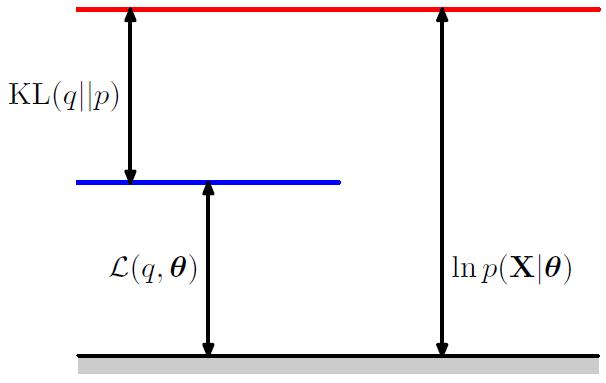
\includegraphics[width=4.5cm]{fig_4_3.jpg}
		\caption{Log-likelihood decomposition.}\label{fig_4_3}
	\end{minipage}
	\begin{minipage}[t]{0.48\linewidth}       
		\centering
		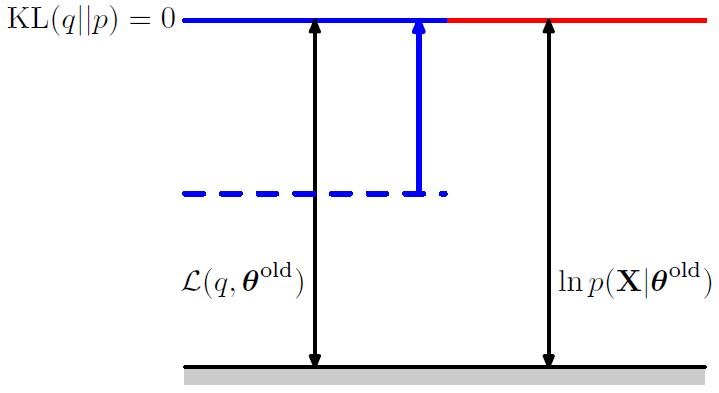
\includegraphics[width=5.4cm]{fig_4_4.jpg}
		\caption{The E step of the EM algorithm.}\label{fig_4_4}
	\end{minipage}
\end{figure}
\par In the E step of the EM algorithm, the lower bound is maximized with respect to $q({\bf Z})$ with $\bm{\theta}=\bm{\theta}^{\text{old}}$ fixed. From (\ref{eq_4_em_in_g_lbdcp}), we can easily see that the maximum is obtained when the KL divergence vanishes since $\ln p({\bf X}|\bm{\theta}^{\text{old}})$ does not depend on $q({\bf Z})$. The E step is illustrated in Figure \ref{fig_4_4}. This means that in the E step, we find the posterior probability $p({\bf Z}|{\bf X},\bm{\theta})$ by maximizing the lower bound $\mathcal{L}(q,\bm{\theta})$ w.r.t. $q({\bf Z})$.
\begin{figure}[h]
	\centering
	\begin{minipage}[t]{0.42\linewidth}
		\centering
		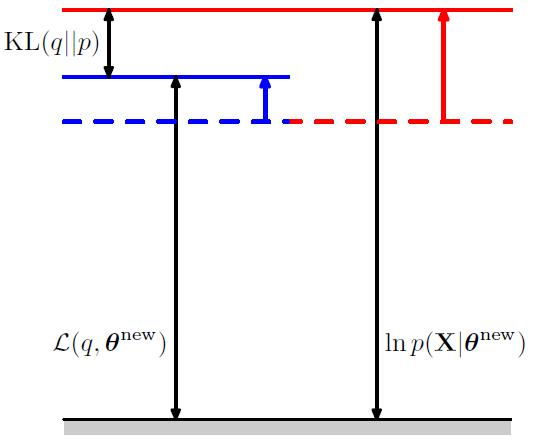
\includegraphics[width=4.5cm]{fig_4_5.jpg}
		\caption{The M step of the EM algorithm.}\label{fig_4_5}
	\end{minipage}
	\begin{minipage}[t]{0.48\linewidth}       
		\centering
		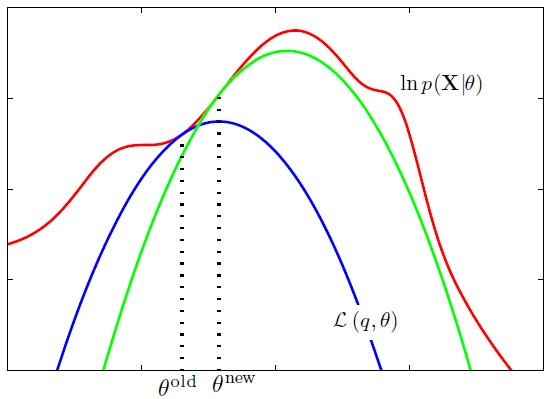
\includegraphics[width=5.4cm]{fig_4_6.jpg}
		\caption{The updates of EM.}\label{fig_4_6}
	\end{minipage}
\end{figure}
\par In the M step, the distribution $q({\bf Z})$ is fixed an the lower bound $\mathcal{L}(q,\bm{\theta})$ is maximized with respect to $\bm{\theta}$ to give some new value $\bm{\theta}^{\text{new}}$. This will cause the lower bound $\mathcal{L}(q,\bm{\theta})$ to increase, and the log-likelihood $\ln p({\bf X}|\bm{\theta}^{\text{new}})$ is therefore increased. However, these two are no longer equal because in general the KL divergence will not be zero after the update. The increase in the log-likelihood is greater than the increase of the lower bound, as shown in Figure \ref{fig_4_5}. If we substitute $q({\bf Z})=p({\bf Z}|{\bf X}, \bm{\theta}^{\text{old}})$ into (\ref{eq_4_em_in_g_lb}), we see that, after the E step, the lower bound takes the form
\begin{align*}
\mathcal{L}(q,\bm{\theta}) &= \sum_{\bf Z}p({\bf Z}|{\bf X}, \bm{\theta}^{\text{old}})\ln p({\bf X, Z}|\bm{\theta}) - \sum_{\bf Z}p({\bf Z}|{\bf X}, \bm{\theta}^{\text{old}})\ln p({\bf Z}|{\bf X}, \bm{\theta}^{\text{old}})\\
&=\mathcal{Q}(\bm{\theta},\bm{\theta}^{\text{old}})+\text{const}
\end{align*}
where the constant is simply the negative entropy of the $q$ distribution and is therefore independent of $\bm{\theta}$. Thus in the M step, we are maximizing the log-likelihood of the complete-data log-likelihood, just as in the case of the Gaussian mixtures.
\par The operation of the EM algorithm can also be viewed in the space of parameters, as illustrated in Figure \ref{fig_4_6}. The red curve represents the (incomplete-data) log-likelihood, which we want to maximize. We begin at some parameter values $\bm{\theta}^{\text{old}}$, and in the E step we evaluate the posterior distribution of the latent variables, which yields $\mathcal{L}(\bm{\theta},\bm{\theta}^{\text{old}})$, whose value equals to the log-likelihood at $\bm{\theta}^{\text{old}}$ (the blue curve). In the M step, we updates $\bm{\theta}$ by maximizing $\mathcal{L}(\bm{\theta},\bm{\theta}^{\text{old}})$, which gives $\bm{\theta}^{\text{new}}$. The subsequent E step then constructs a bound that is tangential at $\bm{\theta}^{\text{new}}$ as shown by the green curve.
\section{Latent Dirichlet Allocation}
\subsection{Motivation}
In the pLSA model, both dimensions of the data matrix are fixed, which means that with pLSA we can only sample words in the vocabulary for existing documents. To sample new documents, one reasonable extension of pLSA is to allow sampling additional rows of the co-occurrence matrix ${\bf X}$, as illustrated in Figure \ref{fig_4_7}. To do this, we need to be able to sample new topic weights ${\bf u}_i=\{u_{1i},\dots,u_{Ki}\}$ for new documents. Combined with a fixed existing topic-to-word matrix ${\bf V}$, we can predict new data rows. This idea motivates the Latent Dirichlet Allocation (LDA), which acts as a Bayesian improvement of pLSA. 
\begin{figure}[h] 
	\centering 
	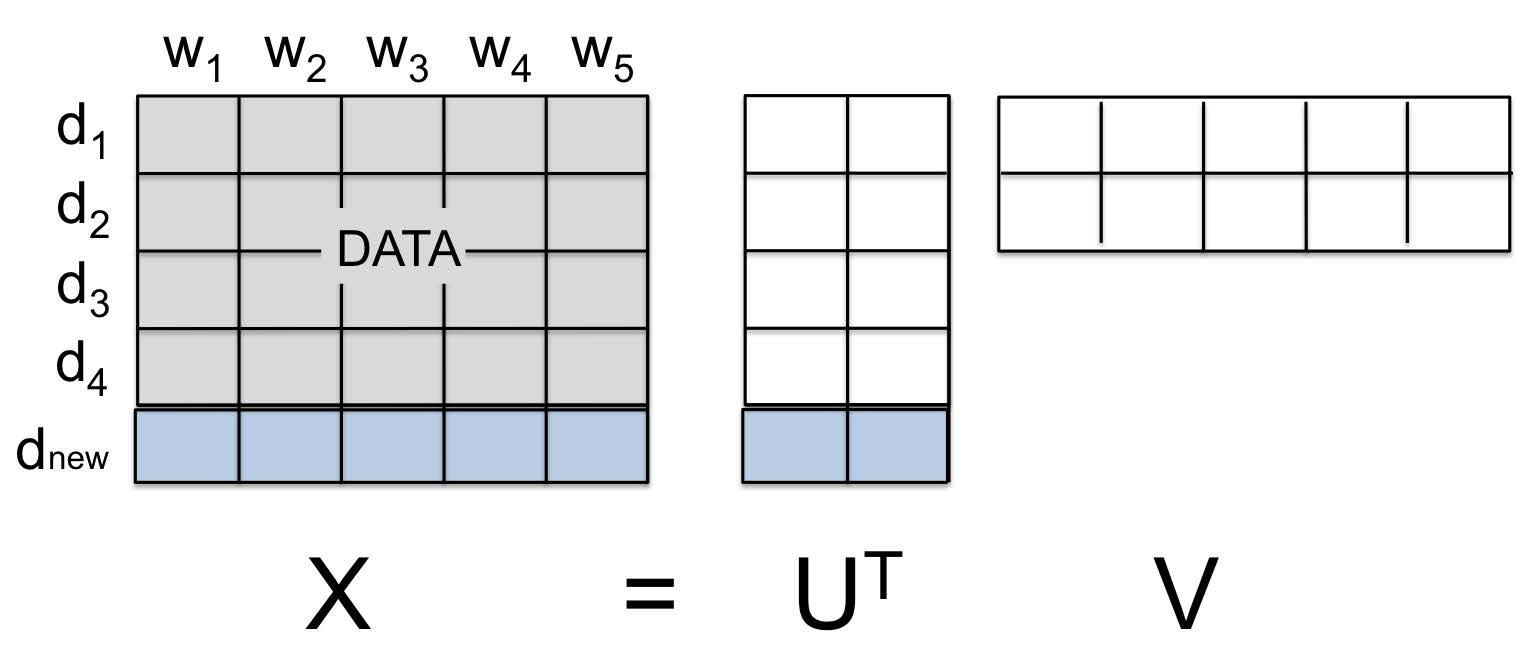
\includegraphics[width=8cm]{fig_4_7.jpg} 
	\caption{We can sample new "documents" by sampling new rows of co-occurrence matrix ${\bf X}$.}\label{fig_4_7}
\end{figure}
\begin{remark}
	If ${\bf X}$ is a count matrix, ${\bf V}$ has to take into account the number of words and can not be a row-normalized probability matrix since we assume $\{{\bf u}_i\}$ are normalized, but if $X_{ij}$ represents $p(w_j|d_i)$, ${\bf V}$ can be a topic-to-word probability matrix. Or, alternatively, we can view the equality in Figure \ref{fig_4_7} as "sampled from".
\end{remark}
\par To sample a new topic weights ${\bf u}_i$, we need to make it a probability vector. The constraints, $u_{ij}\geq 0$ and $\sum_j u_{ij}=1$, indicate that the topics of words that are sampled from ${\bf u}_i$ are subject to a multinomial distribution given a particular document $d_i$. This suggests the choice of Dirichlet distribution as the prior of ${\bf u}_i$ since it's the simplest (conjugate) distribution of a multinomial distribution. The word \emph{conjugate} means a reproducing property: if the prior of parameters is from a Dirichlet distribution with the observations from a multinomial distribution, the posterior distribution of the model parameters will remain a Dirichlet distribution after applying the Bayes rule. Concretely, we have
\begin{equation*}
p({\bf u}_i|\alpha)\propto\prod_{z=1}^{K}u_{zi}^{\alpha_z-1}
\end{equation*}
where $\alpha\in \mathbb{R}^K$ are hyper-parameters that can be used to generate topic weights. Note that traditionally, $\alpha_z$ has a interpretation as a pseudo count of the number of times that topic $z$ is chosen which in the posterior distribution will be added with the actual count. Given $\alpha$ and the Dirichlet assumption, we can already sample new topic weights, but with this Bayesian setting we can benefit from doing model averaging. Specifically, we can treat ${\bf U}$ as nuisance parameters that need to be averaged out, and ${\bf V}$ are real parameters. Note that ${\bf U}$ can be re-constructed, if needed.
\subsection{Model and Algorithm}
The LDA defines a vector of word counts that can be regarded as a new document. Specifically, the LDA model with fixed document length $l=\sum_j x_j$ defines a multinomial observation model that is given by
\begin{equation*}
p({\bf x}|{\bf V, u})=\frac{l!}{\prod_j x_j!}\prod_j \pi_j^{x_j},\ \pi_j := \sum_z v_{zj}u_z
\end{equation*}
where ${\bf x}$ is the word count vector, and $l!/\prod_j x_j!$ is the corresponding normalization factor for a multinomial distribution. Then performing Bayesian averaging over the topic weights ${\bf u}$ yields
\begin{equation*}
p({\bf x}|{\bf V}, \alpha) = \int p({\bf x}|{\bf V, u}) p({\bf u}|\alpha)d{\bf u}.
\end{equation*}
LDA corresponds to the following generative model:
\begin{itemize}
	\item For each document $d_i$: sample ${\bf u}_i\sim \text{Dirichlet}(\alpha)$, where the $\alpha$ are often chosen trivially. Note that the ${\bf u}_i$ will be integrated out in Bayesian averaging when we compute the marginal distribution of word count vectors generated from a LDA model.
	\item For each word slot $w^t,\ 1\leq t\leq l_i$, we do the followings in a i.i.d. manner (therefore we can simply treat all word slots by producting them together):
	\begin{itemize}
		\item Sample topic $z^t \sim \text{Multi}({\bf u}_i)$, which is latent and will be summed out in the marginal distribution of word count vectors generated from this LDA model.
		\item Sample the desired observation $w^t\sim \text{Multi}({\bf v}_{z^t})$.
	\end{itemize}
\end{itemize}
\par There are several algorithms that can be used for LDA. However, since they are beyond the scope of this course, we just list some of them here:
\begin{itemize}
	\item variational expectation maximization
	\item Markov Chain Monte Carlo (MCMC): collapsed Gibbs sampling
	\item distributed, large-scale implementations (100Ms of documents)
\end{itemize}
\section{Non-Negative Matrix Factorization}
As illustrated in Figure \ref{fig_4_7}, pLSA can be regarded as an instance of Non-Negative Matrix Factorization (NMF). Although it seems that we are just add some additional constraints like non-negativity to a standard matrix factorization problem, as we will see in the sequel, NMF has a quite different nature compared with standard MF.
\par In many cases, such as pLSA, we are dealing with a count matrix (take image reconstruction as an example where we do not deal with a count matrix), and we want to model it in a two-set setting (like topic-word and user-item) with some product of probabilities. We first normalize the rows of the count matrix as ${\bf X}\in \mathbb{R}^{N\times M}_{\geq 0}$, and we try to find the NMF of ${\bf X}$:
\begin{equation*}
{\bf X}\approx {\bf U}^T{\bf V},\ x_{ij}=\sum_{z}u_{zi}v_{zj}=\langle{\bf u}_i,{\bf v}_j\rangle\in [0,1]
\end{equation*}
where we have the follow constraints on matrix factors ${\bf U}$ and ${\bf V}$:
\begin{itemize}
	\item Non-negativity: all parameters are probabilities.
	\item Normalization: ${\bf U}$ is $L_1$ column-normalized, and ${\bf V}$ is row-normalized.
\end{itemize}
The approximation quality is measured via log-likelihood of the original count matrix ${\bf X}_{count}\in \mathbb{Z}^{N\times M}_{\geq 0}$. NMF, just as standard MF, acts also as a dimension reduction method since $N\cdot M\gg (N+M)K-N-M$, where the minus terms come from the normalization constraints.
\par There are also variations of NMF, one of which is to do a non-negative matrix approximation, i.e. qualifying the approximation to ${\bf X}$ via quadratic cost function without normalization constraints on ${\bf U,V}$. Specifically, we want to solve the following optimization problem:
\begin{equation}\label{eq_4_NMF_q_obj}
\min_{{\bf U,V}}J({\bf U,V})=\frac{1}{2}\|{\bf X}-{\bf U}^T{\bf V}\|_F^2,\ \text{s.t. } u_{zi},v_{zj}\geq 0\ (\forall i,j,z).
\end{equation}
This is a similar problem as pLSA, but they are different in the sense of
\begin{itemize}
	\item different sampling models: quadratic cost function arises naturally from maximum (log) likelihood estimation with Gaussian random variables, while in pLSA we assume a multinomial distribution on observations;
	\item different objectives: we use quadratic loss instead of KL divergence (for details see the remark below);
	\item different constraints: we do not assume normalized parameters.
\end{itemize}
\begin{remark}
	Maximizing the log-likelihood of pLSA model has another interpretation as minimizing a weighted sum of KL divergences between our model predictions and the empirical data distributions. Recall that the log-likelihood of pLSA takes the form of
	\begin{equation*}
	l({\bf U,v})=\sum_{i}\sum_{j}x_{ij} \ln p(w_j|d_i).
	\end{equation*}
	Define $l_i=\sum_j x_{ij}$ as the number of words in $d_i$, and we can re-write the log-likelihood as
	\begin{align*}
	l({\bf U,v})&=\sum_{i}l_i\sum_{j}\frac{x_{ij}}{l_i}\ln p(w_j|d_i)\\
	&= \sum_{i}l_i\sum_{j} p'(w_j|d_i)\left\{\ln \frac{p(w_j|d_i)}{p'(w_j|d_i)} +\ln p'(w_j|d_i)\right\}\\
	&= -\sum_{i}l_i {\rm KL}(p'_{i}||p_i) + {\rm const}
	\end{align*}
	where $p'(w_j|d_i) = x_{ij}/l_i$ is the empirical probability of $w_j$ in $d_i$, and $p'_i$ and $p_i$ are empirical and predictive distribution of words in $d_i$ respectively. We see that maximizing of the log-likelihood is equivalent to minimizing a weighted sum of KL divergences between $p'_i$ and $p_i$, and the weight factors are numbers of words in documents. Note that the constant term is independent of the model parameters.
\end{remark}
\begin{figure}[h] 
	\centering 
	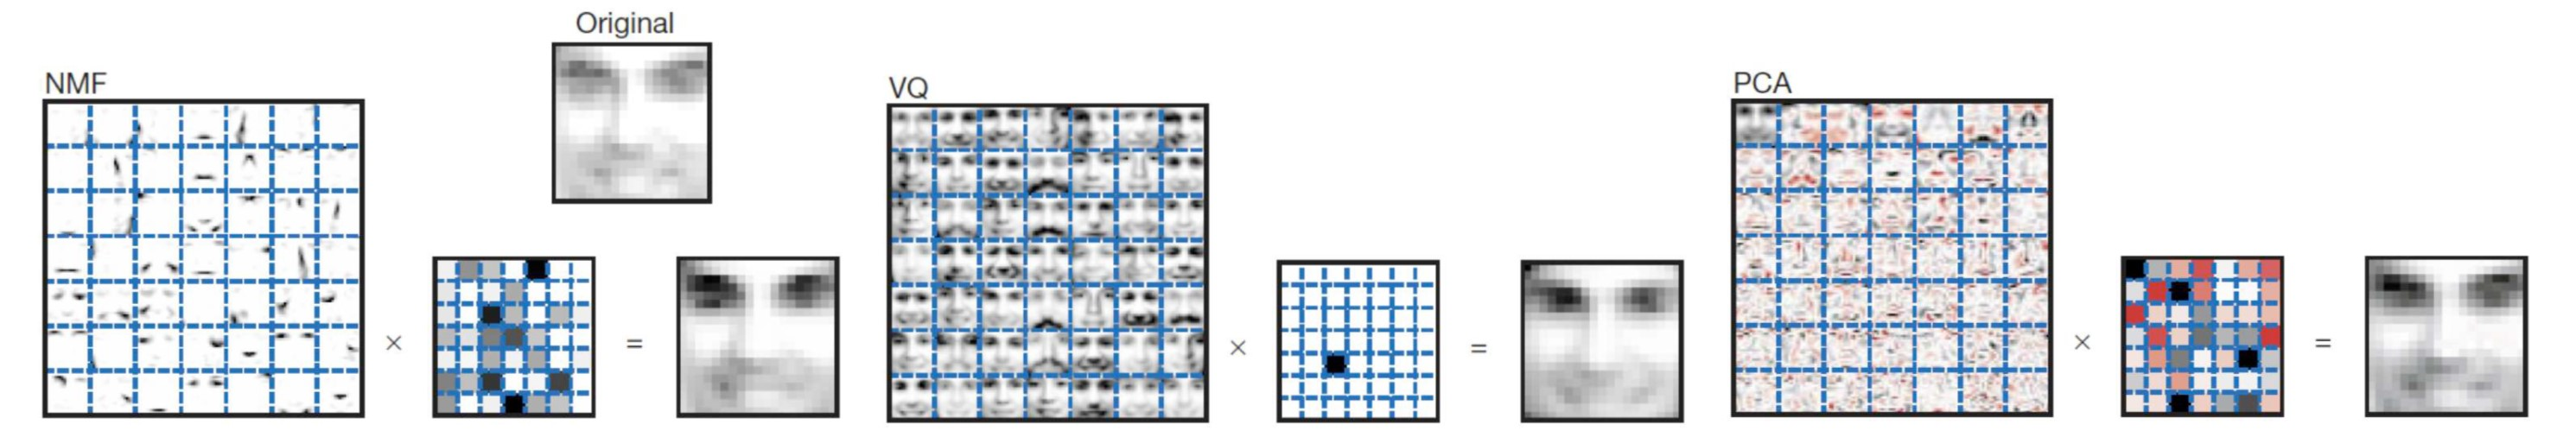
\includegraphics[width=12.5cm]{fig_4_8.jpg} 
	\caption{Different factorization methods for face reconstruction: NMF (left), Vector Quantization (middle), PCA (right).}\label{fig_4_8}
\end{figure}
\par We can see the different nature of factorization methods from the part-based face representation example, as illustrated in Figure \ref{fig_4_8}. NMF is useful when modelling non-negative data (e.g. images, which are non-negative intensities), and since the non-negative constraint requires the model to do additive superpositions without cancellations, NMF learns to represent faces with a set of basis images resembling parts of face, unlike VQ and PCA (see the left picture of Figure \ref{fig_4_8}). However, it is purely a design choice whether to introduce the non-negative constraint.

\par Let us go back to the NMF with quadratic costs and combine things we have covered to see how we can optimize this objective. Since the objective (\ref{eq_4_NMF_q_obj}) is convex in ${\bf U}$ given ${\bf V}$ and vice versa, but not jointly in $({\bf U,V})$, we can choose alternating least squares for optimization. Specifically, we do a alternate optimization of ${\bf U}$ and ${\bf V}$, keeping the other fixed. Given a fixed ${\bf U}$, we can solve for the optimal ${\bf V}$ by re-writing (\ref{eq_4_NMF_q_obj}) as
\begin{align*}
\min_{\bf V}\frac{1}{2}\|{\bf X}-{\bf U}^T{\bf V}\|_F^2 &=\min_{\bf V} \frac{1}{2}\sum_{i,j}(x_{ij}-{\bf u}_i^T{\bf v}_j)^2\\
&=\min_{\bf V}\frac{1}{2}\sum_j ({\bf X}_j - {\bf U}^T{\bf v}_j)^2\\
&=\frac{1}{2}\sum_j \min_{{\bf v}_j}({\bf X}_j - {\bf U}^T{\bf v}_j)^2
\end{align*}
where $\{{\bf X}_j\}$ are columns of ${\bf X}$. Therefore, we can solve for $\{{\bf v}_j\}$ separately, and each of them can be obtained by solving a standard least-square regression type problem. By expanding the square term and setting the derivative w.r.t. ${\bf v}_j$ to zero we get
\begin{equation*}
({\bf UU}^T){\bf v}_j = {\bf UX}_j.
\end{equation*}
Applying the same analysis to ${\bf U}$ and writing the outputs in matrix notations yield the \emph{normal equations} given by
\begin{equation*}
({\bf UU}^T){\bf V} = {\bf UX},\quad \text{and}\quad ({\bf VV}^T){\bf U} = {\bf VX}^T
\end{equation*}
which can be solved via QR-decomposition or gradient descent method. Note that we need to project in between alternations to ensure the non-negativity constraint:
\begin{equation*}
u_{zi} = \max\{0,u_{zi}\},\quad v_{zj} = \max\{0, v_{zj}\}
\end{equation*}
More detailed discussion of algorithms for NMF can be found in Berry, M.W. et al.: Algorithms and applications for approximate non-negative matrix factorization. Computational Statistics \& Data Analysis, 52(1), 2007, pp.155-173.
\par We conclude this chapter with a brief discussion of pLSA and NMF with quadratic loss: \begin{itemize}
	\item They are matrix factorization obeying non-negativity and (optionally, pLSA) normalization constraints.
	\item They have different different cost functions: multinomial likelihood for pLSA, and quadratic loss for NMF (with quadratic loss).
	\item Both of them use a iterative optimization: EM for pLSA, projected ALS for NMF with quadratic loss.
	\item As matrix factorization, they benefit from the interpretability of factors: topics, parts, etc.
	\item They have a wide range of applications.
\end{itemize}
\end{document}